\section{Experimental Validation} \label{sec:c3_experiment}

This section compares experimental forward progress with the modelled one to validate the proposed reactive IPS model and the presented energy storage sizing effects. 

% As the sizing approach suggests the optimal energy storage capacitance in \SIrange{36}{46}{\micro\farad}, we select a \SI{43}{\micro\farad} capacitance in the experiment as an optimal value of the proposed sizing approach for comparison. 
% The forward progress with the optimal capacitance is compared to that with minimum and on-board ones, and an ideal case for a range of supply current. 
% Two goals:
% 1. To validate this model, to show that this model has high accuracy, so it can predict the forward progress reliably, across different energy storage capacitance and supply current. 
% 2. To show that the improvement / optimization of sizing energy storage given different current input conditions (so different energy source conditions). (Given our platform characteristics)

\subsection{Experiment Setup}

We validated our model on the IPS system that we parameterised for exploration (\sref{sec:c3_exploration}), so its IPS method, voltage thresholds, current draws, and workload are as mentioned.
The on-board decoupling capacitance was measured as \SI{10.0}{\micro\farad}, and hence was the minimum capacitance that could be tested. 
Further capacitance was added to provide extra energy storage up to a maximum of \SI{43}{\micro\farad}, as forward progress with this capacitance can approximate \nm{\alpha}{exe\_ideal} (an upper bound), which is linear to supply current \nm{I}{in} when $\nmm{I}{lpm} < \nmm{I}{in} < \nmm{I}{exe}$ (mentioned in \sref{subsec:formulation}).

% === The following paragraph about the actually leakage is a bit weak, so removed for now. ===
% The leakage current of these capacitors was measured to be less than \SI{10}{\nano\ampere} at \SI{3}{\volt}, which is negligible compared to the \SI{}{\micro\ampere}-level current consumption of the platform; hence we omit capacitor leakage in the following experiment and model output. However, this is only applicable to the capacitors and the capacitance range in this experiment; we consider that a leakage model is still necessary for general application.
% the specific leakage current we measured does not deny that \SI{}{\micro\ampere}-level leakage may exist in most electrolytic capacitors;

In practical IPSs, the effective execution time ratio (the metric of forward progress in this chapter) that contributes to the effective output is not easy to differentiate from the execution time that is wasted.
Therefore, in the experiment, the task completion rate, i.e. the number of tasks completed per second, was measured because it directly reflects forward progress and closely relates to the effective execution time ratio.
A task completion was indicated by a positive output pulse from the MCU at the end of a task.
The task completion rate was then obtained by giving an observation window in the oscilloscope that covers a number of output pulses and measuring the frequency of these pulses. 
The task complete rate in the \textit{Intermittent} mode was divided by the one in the \textit{On} mode to obtain the experimental normalised forward progress.

\subsection{Model Validation} 

\begin{figure}
	\centering
	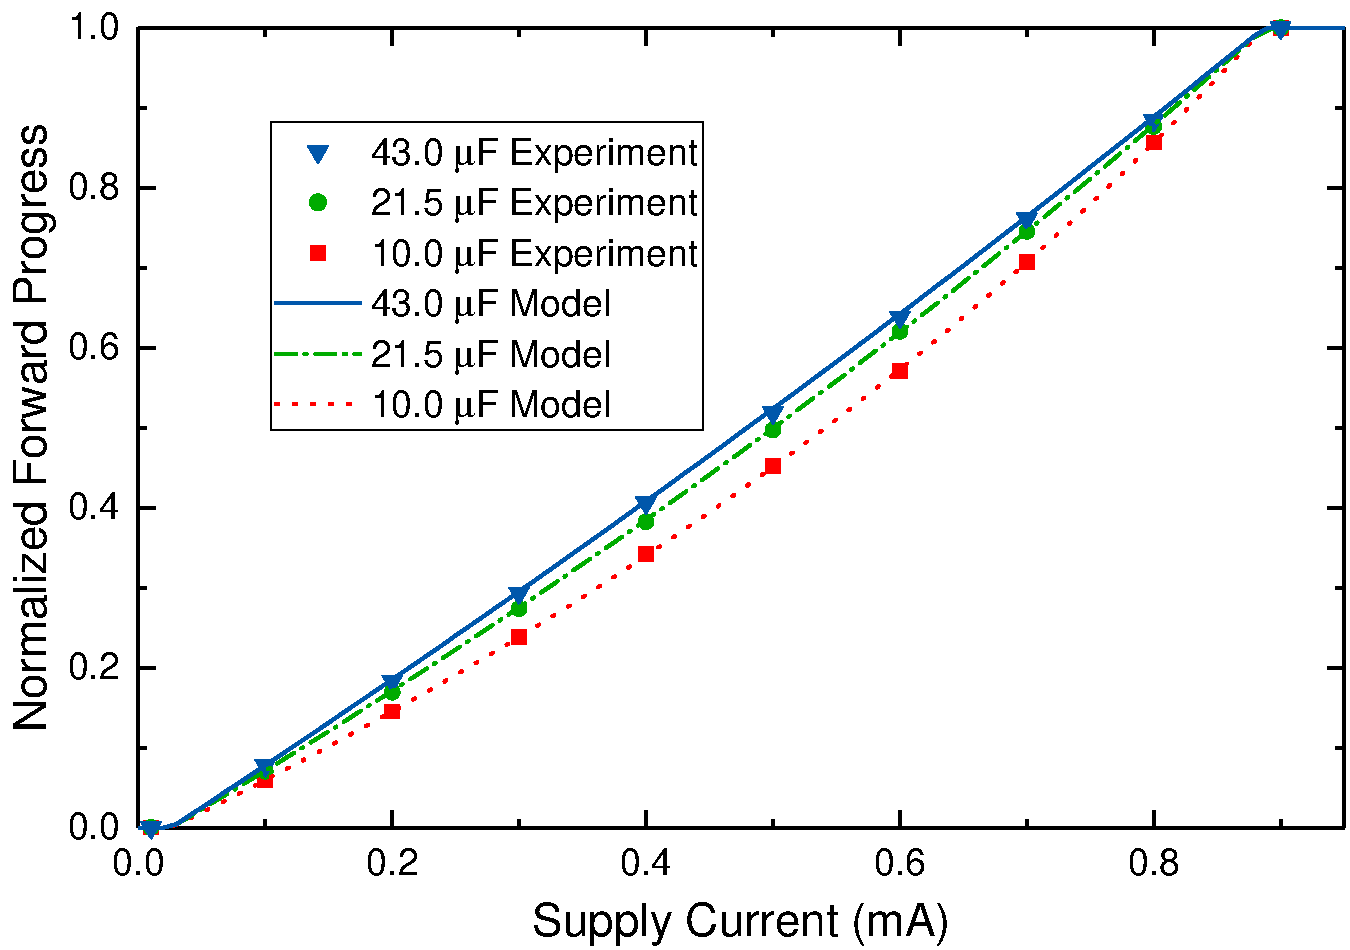
\includegraphics[width=\columnwidth]{ch3_sizingeffect/figures/ModelValidFig}
	\caption{Model validation with experimental and modelled forward progress. }
	\label{fig:modelvalid}
\end{figure}

To validate the accuracy of our model, we powered the device with a range of supply currents (\SIrange{0}{0.9}{\milli\ampere}) to operate the device in \textit{Intermittent} mode, and repeated the tests with three energy storage capacities: a) \SI{10.0}{\micro\farad} decoupling capacitance; b) \SI{21.5}{\micro\farad} (\SI{11.5}{\micro\farad} added); c) \SI{43.0}{\micro\farad} (\SI{33.0}{\micro\farad} added).
We compared the actual forward progress against predictions generated from our model. 
As shown in \figurename{~\ref{fig:modelvalid}}, the model-generated forward progress matches closely with the experimental results with only 0.5\% mean absolute percentage error across all the results. 
Hence, the proposed model is able to accurately estimate forward progress for design exploration. 

\subsection{Validation of Sizing Effects}

\begin{figure}
    \centering
    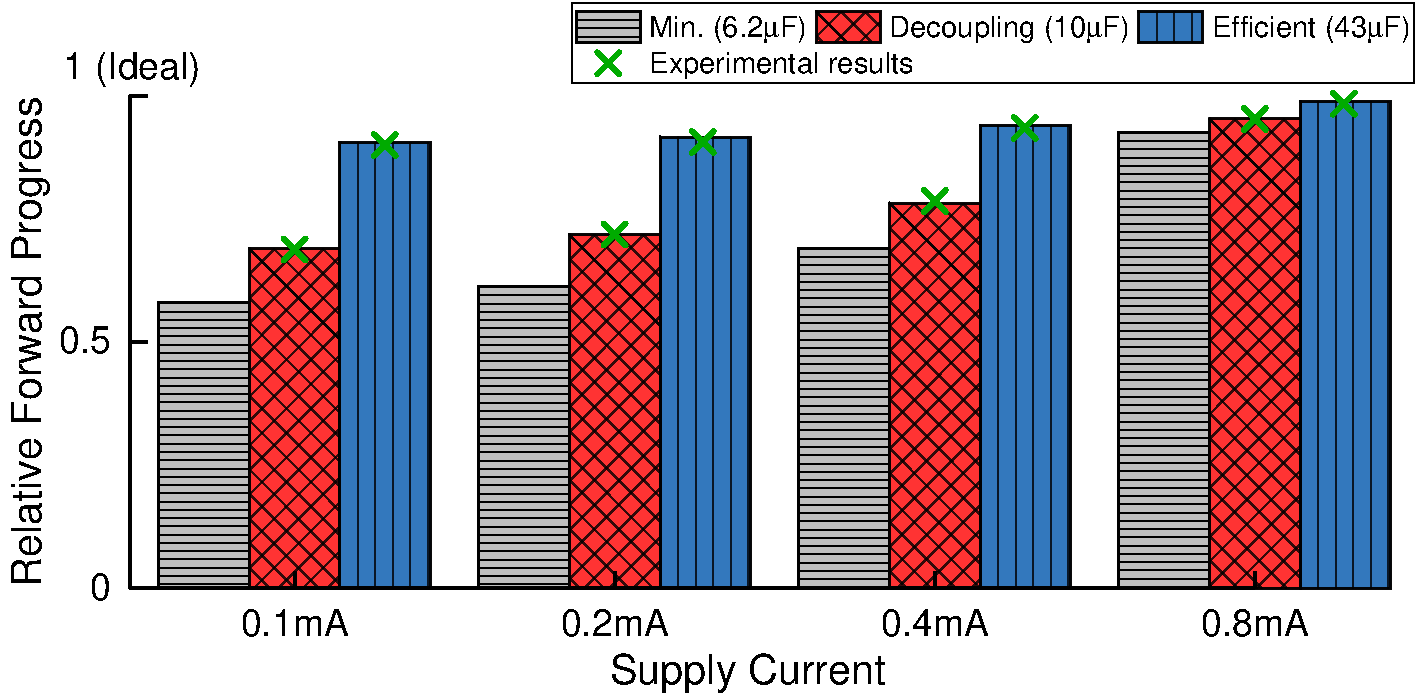
\includegraphics[width=\columnwidth]{ch3_sizingeffect/figures/ImprValidColorFig1}
    \caption{The relationship between energy storage capacitance and IPS forward progress, for various supply currents. }
    \label{fig:imprvalid1}
\end{figure}

As shown with modelled and experimental results in \fref{fig:imprvalid1}, the efficiently-sized energy storage capacitance (\SI{43}{\micro\farad}) improves forward progress by up to 55\% and 30\% compared against using the minimum and decoupling capacitance respectively. 
We notice that this improvement becomes significant when the supply current attenuates because the save and restore overheads consume a larger proportion of the available energy. 
Also, the efficiently-sized capacitor achieves at least 90\% of the ideal forward progress across the tested supply currents.
The ideal case only switches between LPM and execution, without restoring and saving overheads (explained in \sref{subsec:formulation}). 
These results illustrate the importance of this technique, in particular for conditions where the supply current is low.
